\documentclass[12pt,oneside]{book}
\usepackage{geometry}                		% See geometry.pdf to learn the layout options. There are lots.
\geometry{a4paper}                   			% ... or a4paper or a5paper or ... 
%\geometry{landscape}                		% Activate for for rotated page geometry
%\usepackage[parfill]{parskip}    		% Activate to begin paragraphs with an empty line rather than an indent
\usepackage{graphicx}				% Use pdf, png, jpg, or epsß with pdflatex; use eps in DVI mode
								% TeX will automatically convert eps --> pdf in pdflatex		
\usepackage{amssymb}

\usepackage[spanish]{babel}			% Permite que partes automáticas del documento aparezcan en castellano.
\usepackage[utf8]{inputenc}			% Permite escribir tildes y otros caracteres directamente en el .tex
\usepackage[T1]{fontenc}				% Asegura que el documento resultante use caracteres de una fuente apropiada.

\usepackage{hyperref}				% Permite poner urls y links dentro del documento

\title{Mi Juego Favorito}
\author{Javier Tibau}
%\date{}							% Activate to display a given date or no date

\begin{document}
\maketitle
\tableofcontents

\chapter{Introducción}
El libro a continuación es creado como una herramienta para el desarrollo de habilidades de edición colaborativa de documentos de texto plano. La herramienta que habilita dicha colaboración, en este taller, es Git pero podría ser reemplazada por otros sistemas de versionamiento.

\chapter{Los Juegos}

\include{juegos/Buscaminas}
\include{juegos/Dota2}
\include{juegos/Zelda}
\section{Temple Run}

\begin{figure}[htbp]
\begin{center}
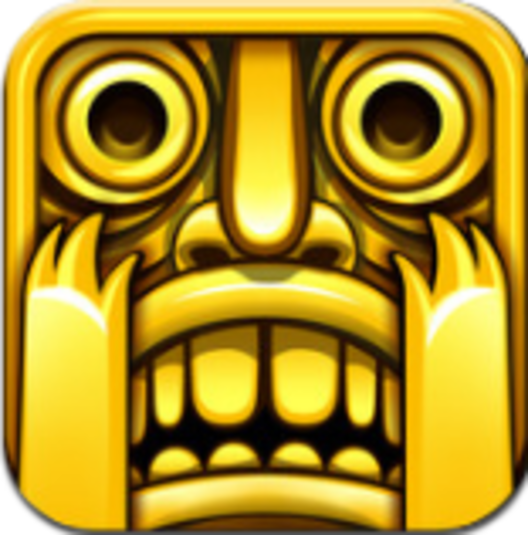
\includegraphics[width=.35\textwidth]{./imagenes/templerun.png}
\caption{Temple Run}
\label{Temple Run}
\end{center}
\end{figure}
En todas las películas de aventuras hay una escena donde el héroe finalmente pone sus manos en el tesoro, pero entonces tiene que atravesar una gran cantidad de trampas para salir vivo. Temple Run\footnote{\url{https://itunes.apple.com/es/app/temple-run/id420009108?mt=8}} es esa escena. Y es asombrosa. Es una de las aplicaciones mas solicitadas tanto en la App Store, como en Google Play por su atractiva interfaz, y por lo divertido de sus niveles. Siéntete como un auténtico buscador de tesoros, y diviértete escapando de los villanos, saltando rampas, esquivando objetos y consiguiendo monedas y poderes.

\subsubsection{¿Por qué es uno de mis juegos favoritos?}
\begin{itemize}
\item[Charlie Medina] Es un juego simple, pero que puede proporcionar horas de entretenimiento. Fue uno de los primeros juegos que descargué cuando consegui un iPhone, y recuerdo que pasé horas jugandolo hasta haber superado los primeros niveles. Lo interesante del juego, es que compites contra ti mismo, ya que lo único que buscas es superar tu propio récord, tratando de llegar cada vez mas lejos, consiguiendo mas monedas (que luego te sirven para comprar objetos) y desbloqueando poderes que te ayudarán a evadir las trampas o que te salvarán de alguna caída, y te permitirán llegar cada vez más lejos. Como el juego no tiene un final, puedes pasar el tiempo que quieras tratando de superarte, y a medidad que llegas mas lejos, se dificulta ya que la velocidad incrementa y tienes que volverte un experto hábil para esquivar objetos a grandes velocidad. Sin duda, recomendado para todos aquellos con smartphones y con bastante tiempo libre.
\end{itemize}
\section{Resident Evil}

\begin{figure}[htbp]
\begin{center}
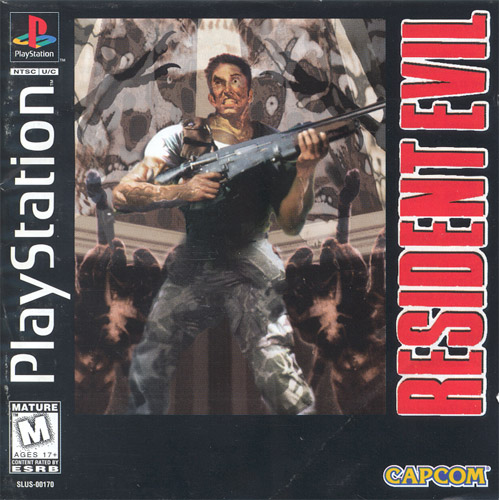
\includegraphics[width=.35\textwidth]{./imagenes/resident_evil1.jpg}
\caption{Resident Evil}
\label{Resident Evil}
\end{center}
\end{figure}
Una extraña ola de asesinatos empiezan a ocurrir en las montañas Arklay a las afueras de Racoon City.  Es entonces que la noche del 24 de julio de 1998 el departamento de policia de Racoon City envia al equipo Bravo del gurpo especial S.T.A.R.S. (Special Tactics And Rescue Service) a investigar. Al poco tiempo se pierde el contacto con el equipo Bravo y se envia al equipo Alpha a continuar la investigacion y encontrar al equipo Bravo. Al llegar son atacados por una especie de perros zombies y son obligados a refugiarse en una mansion cercana. Es Aqui Donde comienza la pesadilla de los S.T.A.R.S. por sobrevivir ya que la mansion es un centro secreto de desarrollo de armas biologicas, y los miembros de S.T.A.R.S. han sido engañados para probar una nueva arma denominada Virus-T la cual es capaz de reviir el tejido muerto a nivel celular. En Resident Evil\footnote{\url{http://www.residentevilcenter.net/residentevil.html}} entramos en la piel de los miembros del equipo Alpha de S.T.A.R.S. Chris Redfield o Jill Valentine los cuales se enfrentaran a monstruos creados con el virus-T tales como zombies y demas criaturas; con municion limitada y su sentido de supervivencia.

\subsubsection{¿Por qué es uno de mis juegos favoritos?}
\begin{itemize}
\item[Joseph Gallardo] Es un juego del genero Survival Horror el cual se caracteriza por su camara estatica, y la escasa municion la cual habra que utilizarla sabiamente, ya que habra ocasiones en las que sera mejor huir antes que pelear. La historia del juego es exelente, los puzzles son un verdadero reto y las desiciones que tomes durante el juego afectan al final de la historia. Es uno de mis videojuegos favoritos ya que lo considero como un verdadero reto para superar.
\end{itemize}


\chapter{Conclusiones}
Cuales juegos fueron más populares y un breve razonamiento del porqué.

\end{document}  
